% Chapter Template

\chapter{Ensayos y resultados} % Main chapter title

\label{Chapter4} % Change X to a consecutive number; for referencing this chapter elsewhere, use \ref{ChapterX}


%----------------------------------------------------------------------------------------
%	SECTION 1
%----------------------------------------------------------------------------------------

En este capítulo se detallan los ensayos realizados para comprobar el correcto funcionamiento de hardware y firmware, y la interacción de los módulos que componen el robot.

\section{Pruebas funcionales del hardware}
\label{sec:pruebasHW}

Para las pruebas funcionales de hardware y software fue necesario completar la construcción mecánica del prototipo, de modo que se pudiera testear el comportamiento del robot frente a obstáculos de distinto tipo. 
En la figura \ref{fig:armado1} se presenta una imagen del prototipo armado y cableado, en estado funcional, sin la tapa superior. 

\begin{figure}[h]
	\centering
	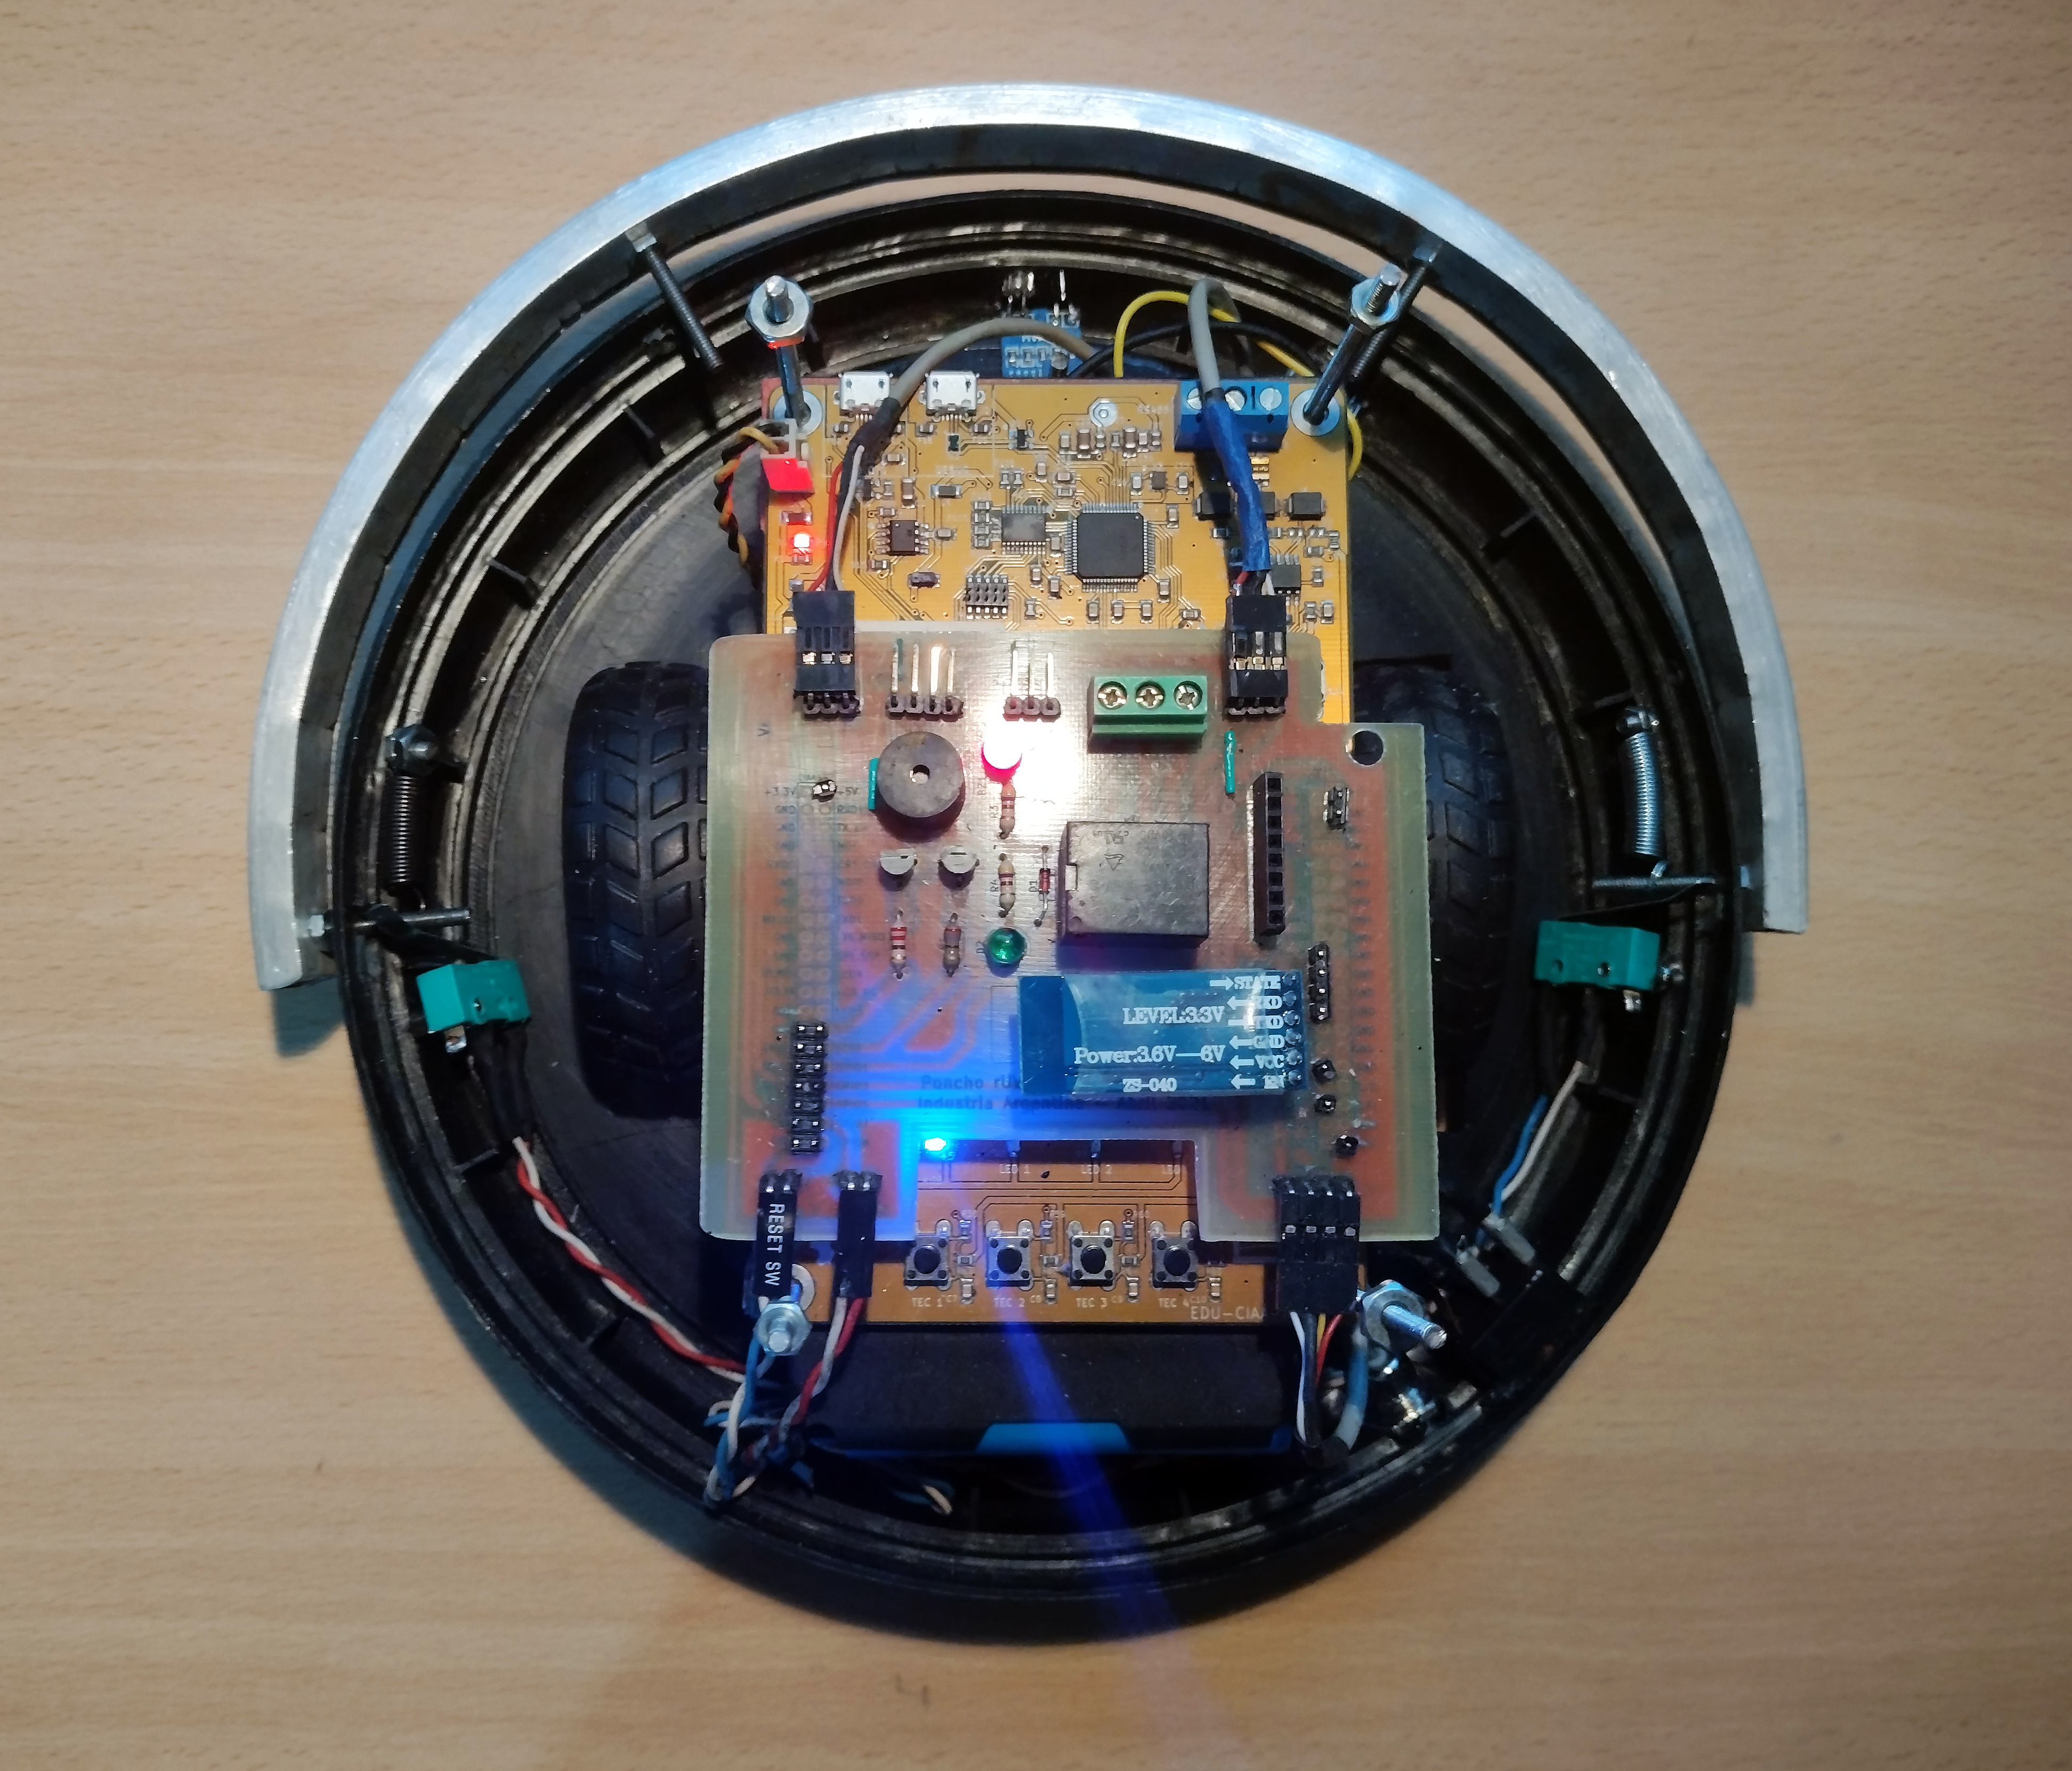
\includegraphics[width=14cm]{./Figures/armado1.jpg}
	\caption{Prototipo armado y cableado, sin la tapa superior.}
	\label{fig:armado1}
\end{figure}

\subsection{Validación de navegación autónoma}
\subsection{Validación de movimientos del robot}
Se verificó que el robot responde a los “estímulos” detectados por los sensores según lo determinado en la librería mde.h, como tabla de configuración de la máquina de estados principal. 
Se utilizaron los LEDs de la placa EDU-CIAA como testigo del estado tomado por la FSM en cada momento. 

\subsection{Validación módulo de comunicaciones Bluetooth}
\subsection{Validación detección de obstáculos}



\section{Pruebas no Funcionales}
%\subsection{Tarea de comunicaciones}